% ****** Start of file apssamp.tex ******
%
%   This file is part of the APS files in the REVTeX 4.2 distribution.
%   Version 4.2a of REVTeX, December 2014
%
%   Copyright (c) 2014 The American Physical Society.
%
%   See the REVTeX 4 README file for restrictions and more information.
%
% TeX'ing this file requires that you have AMS-LaTeX 2.0 installed
% as well as the rest of the prerequisites for REVTeX 4.2
%
% See the REVTeX 4 README file
% It also requires running BibTeX. The commands are as follows:
%
%  1)  latex apssamp.tex
%  2)  bibtex apssamp
%  3)  latex apssamp.tex
%  4)  latex apssamp.tex
%
\documentclass[reprint, amsmath,amssymb, aps, prl]{revtex4-2}

\usepackage{graphicx}% Include figure files
\usepackage{dcolumn}% Align table columns on decimal point
\usepackage{bm}% bold math
%\usepackage{hyperref}% add hypertext capabilities
%\usepackage[mathlines]{lineno}% Enable numbering of text and display math
%\linenumbers\relax % Commence numbering lines
\usepackage{xcolor}
%\usepackage[showframe,%Uncomment any one of the following lines to test 
%%scale=0.7, marginratio={1:1, 2:3}, ignoreall,% default settings
%%text={7in,10in},centering,
%%margin=1.5in,
%%total={6.5in,8.75in}, top=1.2in, left=0.9in, includefoot,
%%height=10in,a5paper,hmargin={3cm,0.8in},
%]{geometry}

\usepackage[utf8]{inputenc}
\usepackage[T1]{fontenc}

\begin{document}

\preprint{APS/123-QED}

\title{Proliferating Tissue With Optical Properties}

\author{Gaston Briozzo$^{1, 2, 3}$}
\author{Fernando Peruani$^{3}$}
\author{Igor Aronson$^{4}$}
%\affiliation{$[1]$ Facultad de Matemática, Astronomía, Física y Computación (FaMAFyC), Universidad Nacional de Córdoba (UNC), Ciudad Universitaria (5000), Córdoba, Argentina,}
%\affiliation{$[2]$ Instituto de Física Enrique Gaviola (IFEG), Consejo Nacional de Investigaciones Científicas y Técnicas (CONICET), Ciudad Universitaria (5000), Ćordoba, Argentina,}
%\affiliation{$[3]$ Laboratoire de Physique Théorique et Modélisation (LPTM) (UMR 8089), Cergy Paris Université (CYU), 2 avenue A. Chauvin, Cergy-Pontoise cedex (95302), France\\}
%\affiliation{$[4]$ Penn state...\\}

\date{\today}

\begin{abstract}
We propose a tissue made up of cells capable of contracting or expanding according to environmental conditions. We develop both a Model Based on Individuals and Hydrodynamic Equations, thus counting on simulations and analytical formalism. The study of the sealing properties of the tissue allows us to determine that it is an elastic liquid. On the other hand, when it is free, the tissue expands producing traveling waves that have optical properties, obeying Snell's law. Furthermore, these waves can be used as a displacement vector for other particles. The model and formalism presented here can be helpful in describing microorganisms such as bacteria that expand colonizing new spaces and consuming resources.
\end{abstract}

%\keywords{Active Matter, Collective Behavior, Emergent Behavior, Environment}
\maketitle

%\tableofcontents

\section{Introduction}

    Active matter studies have advanced significantly in recent decades, allowing for a better understanding of emergent behaviors in systems of interacting mobile agents. These advances have allowed the creation of theoretical models and simulations that describe phenomena such as patterns of self-organization, collective dynamics and responses to external forces. A crucial point in this research is the development of Individual-Based Models (IBMs), which allow simulating the interaction of discrete particles or entities representing biological organisms or their components, with the purpose of investigating the formation and evolution of “tissues” under diverse conditions.

    A paradigmatic IBM model was presented by Peruani et al. in \cite{peruani2008mean} describing pattern formation through spontaneous alignment in moving particles interacting over short distances via cohesive forces. This approach demonstrated the ability of IBMs to capture complex collective dynamics and served as a basis for subsequent work exploring various interaction conditions and confinement geometries. In parallel, Aronson et al. \cite{aranson2006patterns} explored active matter systems under confining conditions and external forces, demonstrating that such systems exhibit viscoelastic properties and phase transitions at the microscopic level. These studies helped to understand how external forces can induce unusual state changes and dynamics in active systems.

    In the present work, we expand the existing knowledge by introducing a novel IBM that models disk-shaped agents interacting through a repulsive potential. This model incorporates elements such as environmental pressure, variable reproduction rate and critical stress, providing a detailed description of the evolution of an active tissue. Unlike previous work, where the focus is on particle alignment or response to external fields, here we consider agents with reproduction and death conditioned by internal and external factors, such as stress and pressure.

    Experiments performed by individual simulations investigate several relevant scenarios. In the steady-state experiment, a single agent placed in a closed vessel is observed to proliferate until it reaches spatial equilibrium, where density, pressure and stress stabilize. This result extends Peruani's work, demonstrating that in more complex confinements, active tissues can reach equilibrium states characterized by minimal fluctuations. The viscoelasticity experiment, on the other hand, shows that the active tissue responds to external forces in a manner similar to a viscoelastic fluid, an observation that complements Aronson's findings on the mechanical properties of active systems.

    Moreover, state-of-matter and wavefront experiments illustrate the complexity of tissue responses under different conditions. State of matter highlights the ability of the tissue to change behavior under constant external forces, while wave fronts reveal the ability of the tissue to transport optical waves with predictable properties through hydrodynamic equations. These phenomena extend the understanding of how active tissues can react and adapt to external perturbations and environmental changes.

    This work represents an advance in the modeling of active matter systems, providing a framework that incorporates critical biological aspects such as reproduction and stress response. By presenting a diversified set of experiments and results, we lay the groundwork for future research exploring the complexity of active tissues in dynamic environments and in response to varying forces and conditions.

\subsection{Model}
\label{Model}

\subsubsection{Individual-Based Model (IBM)}
\label{IBM}

    To model an active tissue that grows and expands, colonizing new regions, but also saturates, depleting resources and shrinking, we propose a system of disk-shaped agents of \textit{radius} $R$ that interact with each other through a \textit{soft-body repulsive potential} $U(r_{ij})$, which penalizes overlaping \cite{PS_2019} and depends on the distance $r_{ij}$ between them. Agents do not move by themselves, i.e., they are not self-propelled, but can be pushed by external forces, such as those exerted by other agents and by the vessel walls.
    Thus, each agent will be exposed to a \textit{pressure} $P$, derived from all the forces acting on it. Agents will move following the pressure gradient, but they will also experience a \textit{stress} $\sigma$, generated by exposure to the pressure at a \textit{stress rate} $\kappa$. This stress can be understood as the pressure accumulated by agents in the last time.
    Free of stress, agents reproduce at \textit{reproductive rate} $r$. 
    However, stress reduces the effective reproduction rate, so that when the \textit{critical stress} $\sigma_c$ is reached there is no reproduction, while if this stress is overcome, the agents will begin to die, with a death rate proportional to the stress.

    The evolution equations for the $i$-th agent are
    \begin{equation}
        \begin{split}
        \dot{\mathbf{x}}_i(t) &= -\gamma \nabla U_i(t), \\
        \dot{\sigma}_i(t)     &= \kappa \left[ P_i(t) - \sigma_i(t) \right], \\
        U_i(t)                &= \sum_{j \in \mathbb{N}_i(t)} U\left[r_{ij}(t) \right] + U_{w}\left[r_{i}(t) \right], \\
        P_i(t)                &= \frac{1}{2\pi R_0} \sum_{j \in \mathbb{N}_i(t)} \left| \nabla U\left[r_{ij}(t) \right] \right| + \left| \nabla U_{w}\left[r_{i}(t) \right] \right|, \\
        p_i(t)                &= r \left[ 1 - \frac{\sigma_i(t)}{\sigma_c} \right],  
        \end{split}
        \label{eq:IBM_EE}
    \end{equation}
    where $\mathbf{r}_{ij}(t)= \dot{\mathbf{x}}_i(t) - \dot{\mathbf{x}}_j(t)$ is the distance vector between agents $i$ and $j$ at time $t$,  $\mathbb{N}_i(t)$ is the set of first neighbors of the $j$-th agent ($j \in \mathbb{N}_i \iff r_{ij}<2R$), $U_{w}$ is the force applied by the walls and $\left| p_i(t) \right|$ is the rate at which the agent reproduces ($0<p_i(t)$) or dies ($p_i(t)<0$) at time $t$. If the agent reproduces, an identical copy of it is generated and placed at a distance $R$ from the original, at a random position. If the agent dies it is removed from the simulation and the space it occupied is freed (it does not leave a corpse).
    Note that all variables have been renormalized to reduce the set of parameters needed.

    

\subsubsection{Partial Differential Equations (PDE)}
\label{PDE} 

    Agents will then move, reproduce and die, making the tissue density a dynamic property.
    In a coarse-grained approximation, we can neglect the particularities of individual agents and consider the tissue as a continuum, whose density at a given position will be given by the probability of finding an agent there.
    Let $\rho(\mathbf{x},t)$ be the agents \textit{probability density} at position $\mathbf{x}$ and time $t$. 
    The \textit{probability current} is written as
    \begin{equation}
        \mathbf{J}(\mathbf{x},t) = - \rho(\mathbf{x},t) \nabla U(\mathbf{x},t) 
        \label{eq:PDE_J}     
    \end{equation}
    Then, the \textit{Fokker-Planck equation} results
    \begin{equation}
        \partial_t \rho(\mathbf{x},t) = r \left[ 1 - \frac{\sigma(\mathbf{x},t)}{\sigma_c} \right]\rho(\mathbf{x},t) + \nabla \left[ \rho(\mathbf{x},t) \nabla U(\mathbf{x},t) \right].
        \label{eq:PDE_FP}     
    \end{equation}
    where $\sigma(\mathbf{x},t)$ and $U(\mathbf{x},t)$ are external fields that depend on $\rho(\mathbf{x},t)$. 
    This leads to the following set of partial differential equations which describe the dynamics of the tissue, often referred to as \textit{hydrodynamic equations}, 
    \begin{equation}
        \begin{split}            
            \dot{\rho}   &= r \left[ 1 - \frac{\sigma}{\sigma_c} \right]\rho + \nabla \left[ \rho \nabla U(\rho) \right] \\
            \dot{\sigma} &= \kappa \left[ P(\rho) - \sigma \right], 
        \end{split}
        \label{eq:PDE_HE}     
    \end{equation}   
    where $P(\rho)$ must be derived from the chosen potential $U(r)$.
    NOTAR: $U$ y $P$ son funciones solo de $\rho$ y $\nabla \rho$.
    Note that these equations turn out to be autocatalytic \cite{hallatschek2023proliferating}.
    
\section{Numerical Results}
\label{NR}

	NOTAR: En lo que siguie se utiliza $P=U$. Esto no es correcto desde el punto de vista de las ecuaciones, pero es lo que se utilizó para realizar las simulaciones

    From now on, unless explicitly stated otherwise, we will use the following parameters
    \begin{equation}
        \begin{split}
            R         &= 1, \\
            r         &= 0.1, \\
            \kappa    &= 0.001, \\
            \sigma_c  &= 0.25,
        \end{split}
        \label{eq:Parameters}
    \end{equation}
    and the following soft potential
    \begin{equation}
        U(r_{ij}) = \left\{
	       \begin{array}{ll}
		   \frac{R_0}{r_{ij}} + \frac{R_0}{R_c^2}r_{ij} - 2\frac{R_0}{R_c},      & \mathrm{if\ } r_{ij} < R_c \\
		   0,                                                                    & \mathrm{if\ } R_c \leq r_{ij} 
	       \end{array}
	     \right. ,      
        \label{eq:Potencial}
    \end{equation}
    being $R_0=R$ a parameter for modeling the potential and $R_c=2R$ the cutoff radius, which indicates the maximum range of the interactions. We emphasize that the same phenomenology studied here can be obtained using other stronger potentials, such as the Lennard-Jones. The choice of a softer potential is based only on the fact that it facilitates the numerical implementation. The whole analytical and phenomenological development is equally valid for any repulsive potential.

\subsection{Stationary}
\label{Stationary}

\subsubsection{Stationary State}
\label{SS}

    The system consists of a dynamic tissue that expands under suitable conditions, colonizing empty spaces. However, under pressure the cells that compose it die, so the tissue contracts.
    We may wonder what will happen then with a tissue confined in a closed vessel. Will a static equilibrium be reached or will we see a periodic behavior?

    In the following experiment, we leave a single cell in a closed square vessel of side $L_v=200$. The tissue proliferates freely until it reaches the edges of the vessel, at which point the pressure increases, contracting the tissue. As the cells die, space is freed and the pressure decreases, triggering a new growth pulse. This behavior is reproduced periodically, although it attenuates with time.

    \begin{figure}
        \centering
        \includegraphics[width=4.2cm,trim=0 0 0 0]{Images/NvsT.pdf}
        \includegraphics[width=4.2cm,trim=0 0 0 0]{Images/PvsT.pdf}
        \includegraphics[width=4.2cm,trim=0 0 0 0]{Images/HvsT.pdf}
        \includegraphics[width=4.2cm,trim=0 0 0 0]{Images/SvsT.pdf}
        \includegraphics[width=8.0cm,trim=0 0 0 0]{Images/All.pdf}
        \caption{
        Asymptotic state. 
        The top four figures show the time evolution of density $\rho$, pressure $P$, tress $\sigma$ and hexatic order $H$ in blue for a vessel of side $200$ and in yellow for a vessel of side $1000$. The initial condition is a single particle inside a closed square vessel. We can see that the values tend asymptotically to equilibrium, presenting small oscillations due to size effects that decrease with time.
        In the bottom figure we can see the relative phase of the different observables. It can be seen that the phases of density and pressure coincide while they are at half phase of the hexatical order and at quarter phase of the stress.
        }
        \label{fig:SS}
    \end{figure}

    The exatic order $H$ gives a measure of how closely the tissue resembles a hexagonal lattice and is defined for the $j$-th agent as
    \begin{equation}
        H_j(t) = \frac{1}{ \| \mathbb{N}_j(t) \|} \sum_{k \in \mathbb{N}_j(t)} e^{i \theta_{jk}(t)}
        \label{eq:HO}
    \end{equation}
    where $\mathbb{N}_j(t)$ is the set of first neighbors of the $j$-th agent, $i$ is the imaginary unit and $\theta_{jk}$ is the angle between the agents $j$ and $k$.

    Fig. \ref{fig:SS} shows density $\rho$, hexatic order $H$, pressure $P$ and stress $\sigma$ as a function of time $t$. The behavior of these quantities can be understood as the sum of two different phenomena. First, a mean value that decays asymptotically to an equilibrium value, in a characteristic time close to $\kappa$. Second, oscillations around this mean value, whose frequency and amplitude also decay asymptotically to non-zero equilibrium values. Therefore, a stationary state with small periodical fluctuations is reached.
    However, it can be shown that these oscillations are due to finite size effects. In the thermodynamic limit, when the system size tends to infinity, the amplitude of the oscillations decays to zero, so that all quantities asymptotically approach their equilibrium values.

    It can be seen that both pressure $P$ and stress $\sigma$ tend to the critical stress $\sigma_c$. On the other hand, the hexatic order $H$ indicates that the cells tend to arrange themselves in a regular hexagonal lattice. Using this information, we can calculate the equilibrium density in the following way
    \begin{equation}
        \rho_c = \left[ \frac{\sqrt{3}}{2}r_c^2 \right]^{-1}
        \label{eq:rc}
    \end{equation}
    where $r_c$ is a distance such that $U(r_c)=\sigma_c/6$, so that having $6$ neighbors at a distance $r_c$ located hexagonally, pressure and stress result equal to $\sigma_c$.
    The value of $r_c$ must be derived from the chosen potential, being for our case $r_c=1.5R$.
    Thus, we can write the following state equation
    \begin{equation}
        PV = N \frac{\sigma_c}{\rho_c}, 
        \label{eq:StateEquation}
    \end{equation}
    being $V$ is the volume and $N$ the number of agents, which depends only on the parameter $\sigma_c$.
    In this way, we can predict all the equilibrium state values.    

    If we look at the phase of the oscillations, we can see that the density and pressure are in phase, while the hexatic order has opposite phase and the stress is in counterphase. We can then express $\dot{\rho} \sim \dot{P} \sim -\dot{H} \sim \ddot{\sigma}$. 

    Through the stability analysis of Eq. \eqref{eq:PDE_HE} we find that the point $ \left(\rho, \sigma \right)_0 = \left(0,0\right) $ is a saddle point, with Jacobian 
    \begin{equation}
    \mathbb{J}_0 = \left(
        \begin{array}{cc}
            r & 0 \\
            0 & -\kappa
        \end{array}
        \right)
        \label{eq:J0} 
    \end{equation}
    while the point $ \left(\rho, \sigma \right)_c = \left(\rho_c,\sigma_c\right) $ is a stable spiral with Jacobian 
    \begin{equation}
    \mathbb{J}_c = \left(
        \begin{array}{cc}
            0 & -r \frac{\rho_c}{\sigma_c} \\
            \kappa \left. \frac{\partial P}{\partial \rho} \right| _{\rho_c} & -\kappa
        \end{array}
        \right),
        \label{eq:Jc} 
    \end{equation}
    so that the phase portrait will show orbits decaying asymptotically to the fix point $\left(\rho_c,\sigma_c\right)$. A phase portrait can be seen in Fig. \ref{fig:HE_PP}.
    Thus, the results provided by IBM and the HEs coincide.

    \begin{figure}
        \centering
        \includegraphics[width=8.0cm,trim=0 0 0 0]{Images/HE_SS.pdf}
        \caption{
        Phase portrait and orbit, Eq. \eqref{eq:PDE_HE}.
        The gray arrows indicate the temporal evolution of the system, while the blue line is a particular orbit that starts near the saddle point $(0,0)$ and ends at the stable spiral $(\rho_c,\sigma_c)$.
        }
        \label{fig:HE_PP}
    \end{figure}

\subsubsection{Viscoelasticity}
\label{VE}

    \begin{figure}
        \centering
        \includegraphics[width=8.0cm,trim=0 0 0 0]{Images/VE_xbvsT.pdf}
        \includegraphics[width=8.0cm,trim=0 0 0 0]{Images/VE_vvsT.pdf}
        \includegraphics[width=8.0cm,trim=0 0 0 0]{Images/VE_FavsT.pdf}
        \caption{
        Viscoelasticity.
        In the upper graph we can see the position of the sphere as a function of time. We see that the amplitude of the displacement is inversely proportional to the frequency of the force.
        In the center image we can see the velocity of the sphere as a function of time. This is more or less in phase with the force and its amplitude does not depend too much on it. In addition we see jumps in the velocity that are due to small voids generated within the tissue.
        In the image on the bottom we see the force exerted by the tissue on the sphere. It can be seen that this is practically equal and opposite to the external force.
        }
        \label{fig:VE}
    \end{figure}  

    Now that we know that we have a tissue in equilibrium, we would like to know its material properties as well. An interesting question may be how the tissue will interact with an foreign body immersed on it. To answer this question we must study the viscoelastic properties of the material.

    In the following experiment, we immerse a solid and rigid sphere of radius $R_s=50$ and mobility $m=0.02$ in the center of a box of sides $L_x=600$ and $L_y=200$ filled with agents in equilibrium. The sphere was subjected to a periodic force $F_{s}(t)=A\cdot \sin \left( \omega t \right)$ in the $x$ direction, repeating the experiment for different frequencies $\omega$. 
    We measured the displacement of the sphere, its velocity and the forces that the tissue exerted on it.

    In the top graph of Fig. \ref{fig:VE} it can be seen how the position of the sphere oscillates due to the periodical external force. In the middle graph, we can see that the velocity of the sphere is almost in face with the external force, depending on the frequency. Finally, in the bottom graph, we see that the the force that the tissue exerts on the sphere is opposite to the external force, $F_{t} \approx F_{s}$.

    In the middle graph it can be seen that, for the higher frequencies, there are indications of collisions between the sphere and the tissue, which are shown as sudden changes in the velocity derivative. This is a consequence of the fast velocity changes of the sphere. The tissue that was behind the sphere did not have time to fill the space left behind. When the sphere changes direction, it moves without resistance for a brief instant before colliding with the tissue. Moreover, when this happens, the tissue that was in the front presses against the sphere, accelerating it even further.

\subsubsection{Matter State}
\label{MS}

    We can now ask whether this tissue behaves as a liquid or as a solid. In the following experiment we let a sphere of radius $R_s=50$ and mobility $m=0.02$ pass through a closed vessel filled with tissue in equilibrium. The sphere is under the effect of a constant force $F_{s}$ pulling it in the $x$ direction. The experiment was repeated by varying the magnitude of $F_{s}$. The results show that, if the magnitude of the force is sufficient, the sphere sinks into the tissue, passing through it as if it were a liquid. However, if the force is small, the sphere will remain floating on the surface. 

    \begin{figure}
        \centering
        \includegraphics[width=8.0cm,trim=0 0 0 0]{Images/ms_xbvsT.pdf}
        \includegraphics[width=8.0cm,trim=0 0 0 0]{Images/ms_vvsT.pdf}
        \includegraphics[width=8.0cm,trim=0 0 0 0]{Images/ms_vvsF.pdf}
        \caption{
        Matter State.
        The top figure shows the position of the sphere as a function of time, the middle figure shows the velocity of the sphere as a function of time and the bottom figure shows the terminal velocity of the sphere as a function of the applied force. It can be seen that if the force is smaller than $F_c$, the sphere will remain floating on the surface, while if the force is larger, the sphere will sink into the tissue. The velocity is proportional to the applied force, following a power law with exponent $3/4$.
        }
        \label{fig:MS}
    \end{figure}  

    Fig. \ref{fig:MS} shows the position of the sphere $x_s$ as a function of time in the top graph, the velocity of the sphere $v_s$ as a function of time in the middle graph and the terminal velocity of the sphere as a function of $F_{s}$ in the bottom graph. If $F_{s}$ is too small, the sphere will remain floating on the surface. If $F_{s}$ exceeds a certain threshold, the sphere will sink. We can see that, as it begins to sink, the sphere moves at a slower velocity. When it is completely sunk, the sphere reaches the terminal velocity $\langle v_s \rangle$, which is higher. This is due to the pressure exerted by the tissue agents on the back of the sphere, propelling it forward.

    In the bottom graph we can see that there is a discontinuous phase transition between the spheres that float and the spheres that sink. The critical magnitude of $F_{s}$ can be estimated as 
    \begin{equation}
        F_c = 2\frac{R_s}{r_c} h \nabla U(r_c),
        \label{eq:MS_Fc}
    \end{equation}
    where $2\frac{R_s}{r_c}$ is the average number of agents that the sphere pushes in the $x$ direction and $h \nabla U(r_c)$ is the average force that these agents receive from their neighbors in the $x$ direction opposite to the sphere, so there is a force balance. 
    We have estimated $h=\left[ 1+2\cos(\frac{\pi}{3}) + 2\cos(\frac{\pi}{6}) \right]\frac{1}{2}$ which is the average of the x-projection of the first neighbors in the two most probable orientations of the hexagonal lattice. This results in $F_c=24.2$, which coincides with the experimental results.
    Moreover, it can be seen that when $F_{s}$ is bigger than $F_c$, the terminal velocity $v$ of the sphere follows a power law, being 
    \begin{equation}
        v(F_{s})=\frac{\pi}{10}m F_{s}^{3/4},
        \label{eq:v(F)}
    \end{equation}
    leading to 
    \begin{equation}
        F_t=\left(1-\frac{\pi}{10} F_s^{-1/4}\right)F_s,
        \label{eq:Ft}
    \end{equation}
    which is consistent with previous results, $F_r\approx F_s$.

    Thus, we can conclude that the tissue behaves like a viscoelastic liquid.

\subsubsection{Pressure}
\label{Ps}

    To correctly describe the properties of the tissue, it is necessary to understand the relationship between density and pressure.
    In the following experiment we will measure the tissue pressure as a function of agent density. For this, we will use a closed square vessel of side $200$ with a fixed number of mobile agents, i.e., the agents interact with each other but cannot reproduce or die. The experiment will be repeated varying the number of agents, thus obtaining the tissue pressure as a function of density.

    \begin{figure}
        \centering
        \includegraphics[width=8cm,trim=0 0 0 0]{Images/pressure.pdf}
        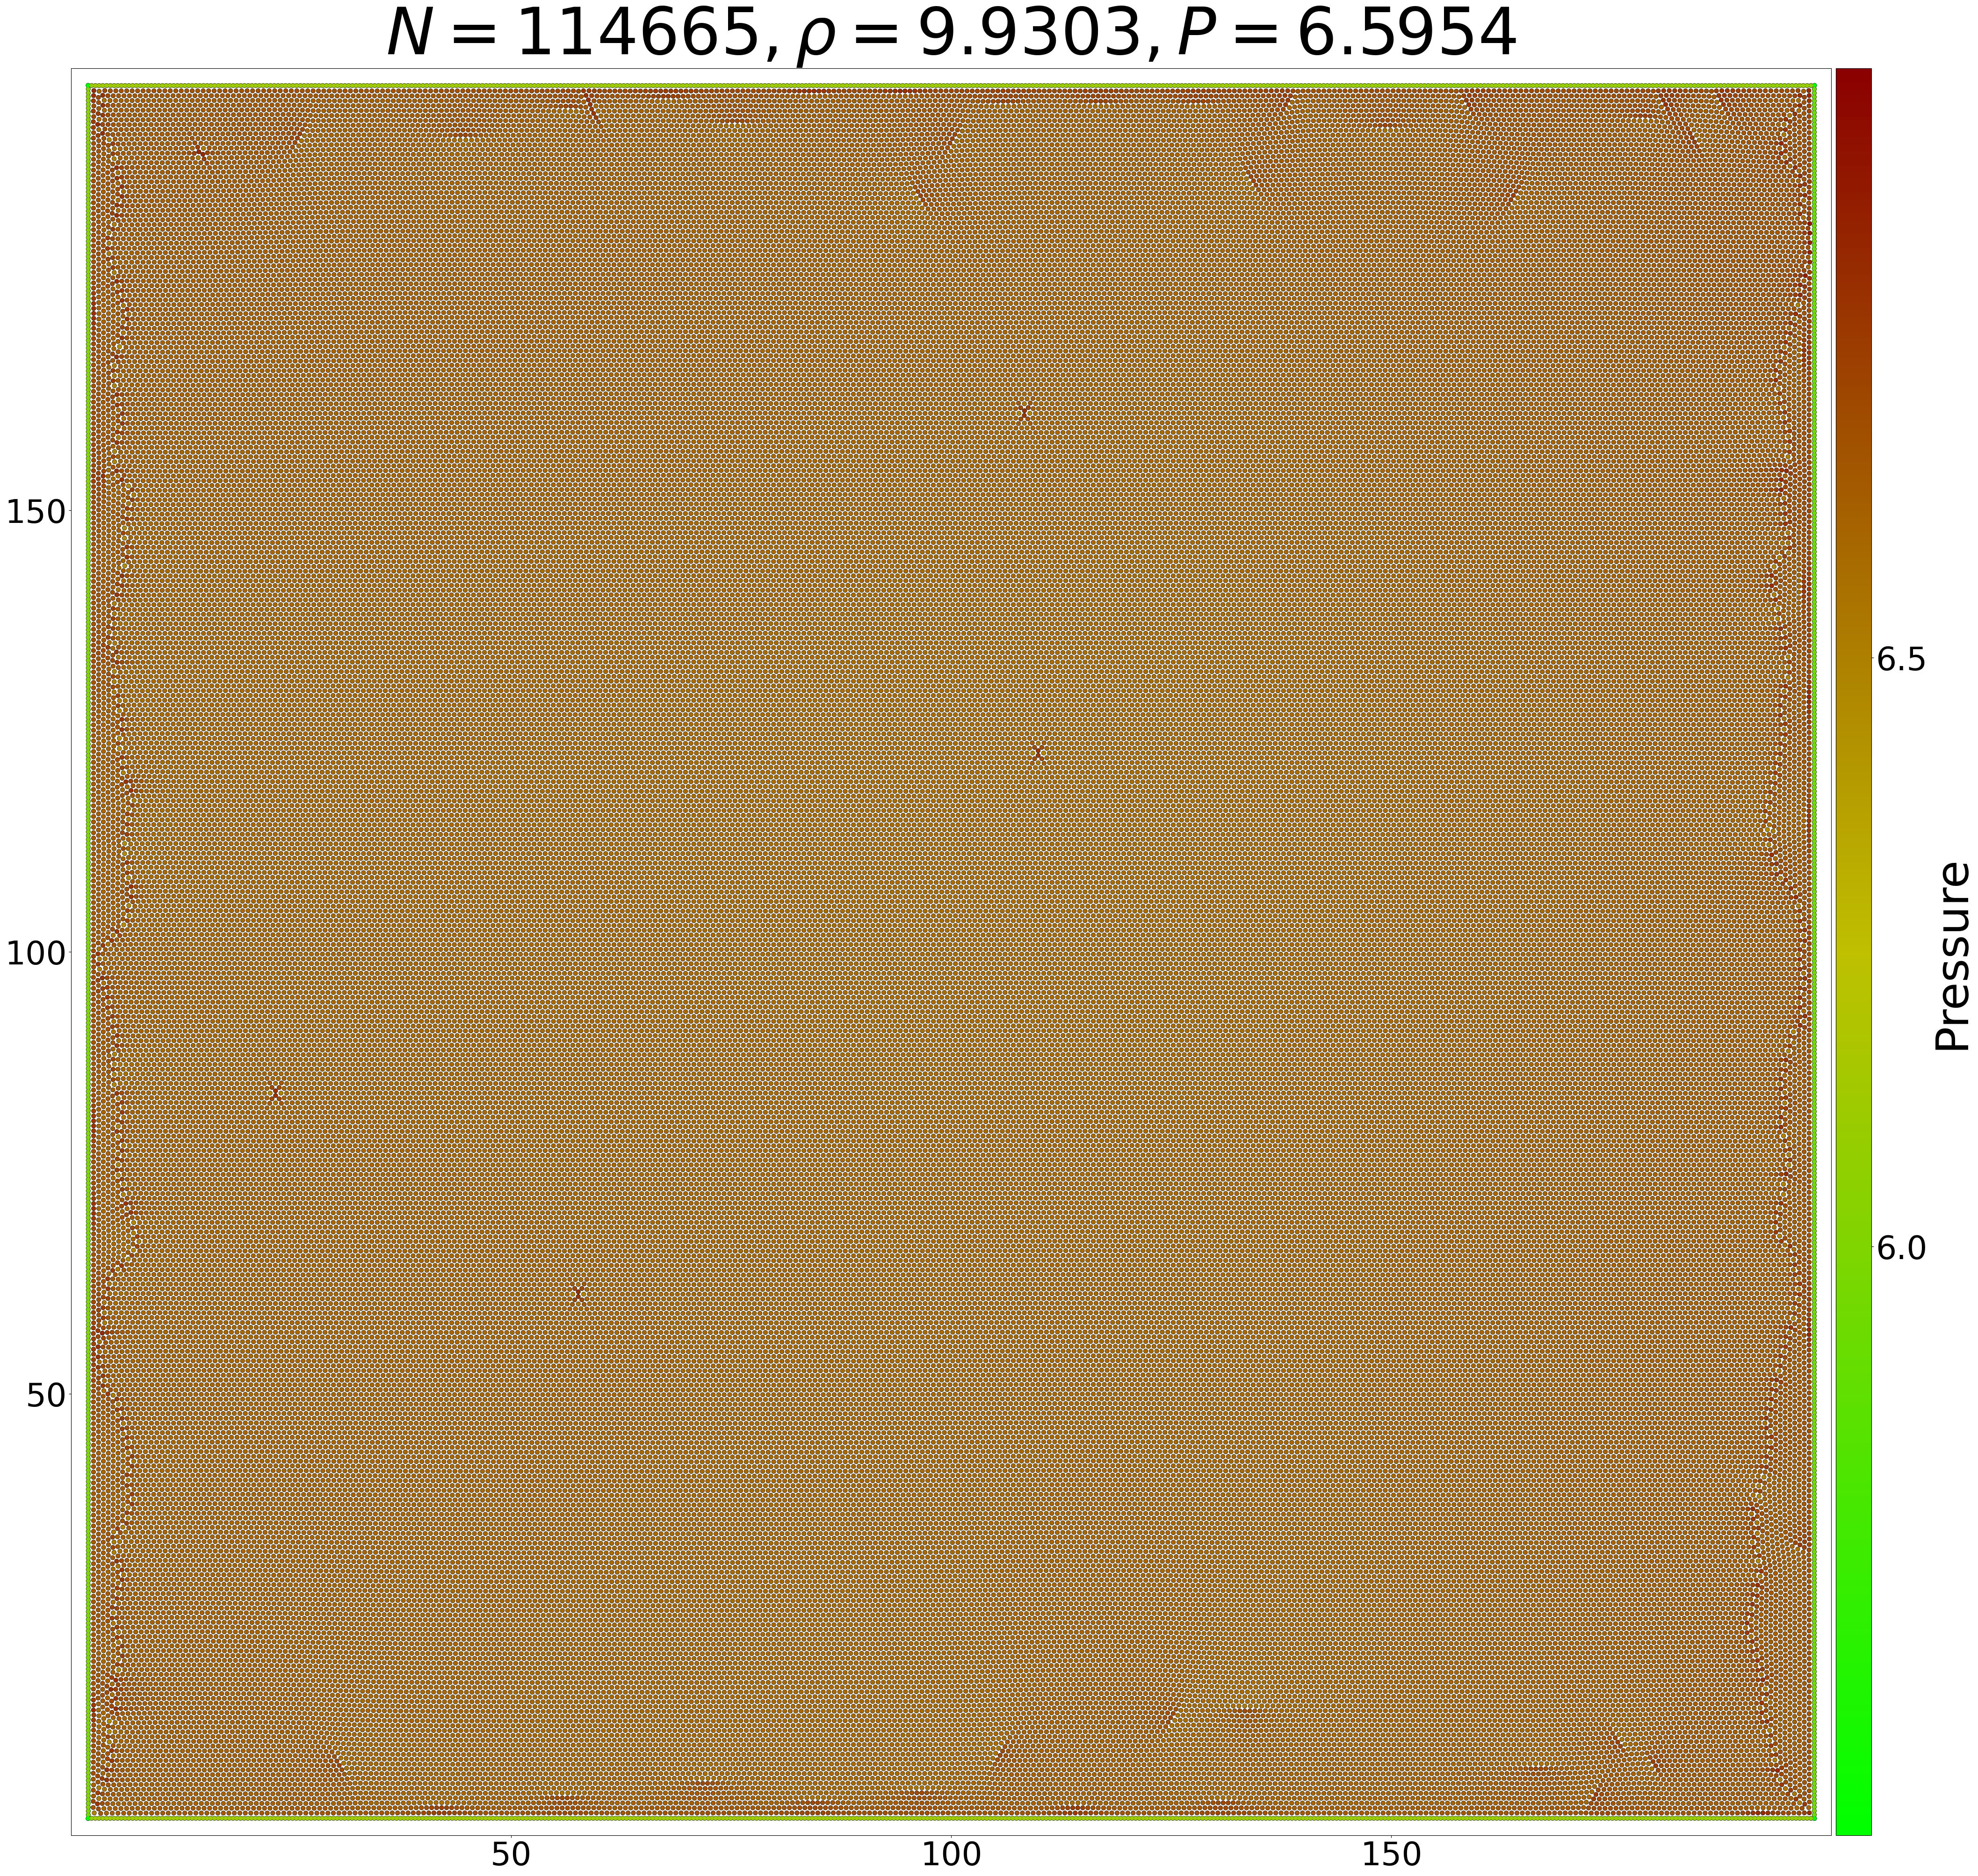
\includegraphics[width=8cm,trim=0 0 0 0]{Images/Pressure.png}
        \caption{
        Pressure.
        The top graph shows the pressure of the tissue as a function of density. 
        Experimental results are shown as dots while theoretical predictions, Eq. \eqref{eq:P(r)}, are shown as a solid line.
        It can be seen that, below a threshold density $\rho_0$, the pressure is zero. Above this density, the pressure increases almost linearly.
        In the bottom graph we can see how the agents are accommodated in an exagonal lattice under extreme pressures.
        }
        \label{fig:Ps}
    \end{figure} 

    The pressures obtained are homegenous within the vessel and boundary effects affect only locally the shape of the lattice, which is hexagonal in most of the system.
    In Fig. \ref{fig:Ps} it can be seen that the pressure is zero for $\rho \leq \rho_0$, being $\rho_0=\rho_c r_c^2/R_c^2$ the density of an exagonal lattice with distance $R_c$ between agents. For higher densities, the pressure can be expressed as
    \begin{equation}
    \begin{split}
        P(\rho) \approx &P_{1}            \left[ \frac{\rho}{\rho_0} -1 \right] \\
                - &P_{-\frac{1}{2}} \left[ \left(\frac{\rho} {\rho_0}\right)^{-\frac{1}{2}} -1 \right] \\
                - &P_{+\frac{1}{2}} \left[ \left(\frac{\rho}{\rho_0}\right)^{+\frac{1}{2}} -1 \right],
    \end{split}
        \label{eq:P(r)}
    \end{equation}
    being $P_{1}$, $P_{-\frac{1}{2}}$ and $P_{+\frac{1}{2}}$ constants. This expresion is derived from the assumption
    \begin{equation}
        P(\rho) = \int_0^{2\pi} \int_{\sqrt{\frac{\rho_0}{\rho}}R_c}^{R_c} \rho U(r) r d\theta dr.
        \label{eq:PU}
    \end{equation}
    This relationship is almost linear and allows to easily determine the pressure as a function of density.

\subsection{Dynamic}
\label{Dynamic}

    In the previous section we studied an equilibrium tissue confined within a closed vessel, but what would happen if the tissue could expand freely?
    Without walls exerting pressure on it, the tissue expands in all directions, producing a circular colonization front. This means traveling wavefronts with optical properties. 

    To study the properties of these waves, in the following experiments we will start with a homogeneous layer of agents at the bottom of a vessel open at the opposite extreme, so that the tissue will expand forming plane waves.    
    These wavefronts exhibit oscillations in density and pressure, which are correctly predicted by the hydrodynamic equations in Fig. \ref{fig:HE_WF}.

    \begin{figure}
        \centering
        \includegraphics[width=4.2cm,trim=0 0 0 0]{Images/HE_KG_d.pdf}
        \includegraphics[width=4.2cm,trim=0 0 0 0]{Images/HE_WF.pdf}
        \includegraphics[width=4.2cm,trim=0 0 0 0]{Images/IBM_KG_d.pdf}
        \includegraphics[width=4.2cm,trim=0 0 0 0]{Images/IBM_WF.pdf}
        \caption{
        Traveling Waves.
        Top row corresponds to HE while bottom row corresponds to IBM. 
        The left column shows density kymographs, where propagating wave fronts can be seen, presenting large oscillations at the front of the wave that attenuate towards the back.
        The right column shows snapshots of density, pressure and stress as a function of position. Here the wavefront oscillations can be better seen.
        Both HE and IBM results are consistent.
        }
        \label{fig:HE_WF}
    \end{figure}  

\subsubsection{Wave Velocity}
\label{WV}

    The velocity of the front depends on the parameters $r$, $\kappa$ and $\sigma_c$, as shown in Fig. \ref{fig:WF_v}.
    \begin{figure}
        \centering
        \includegraphics[width=8.0cm,trim=0 0 0 0]{Images/vvsr.png}
        \includegraphics[width=8.0cm,trim=0 0 0 0]{Images/vvsk.png}
        \includegraphics[width=8.0cm,trim=0 0 0 0]{Images/vvss.png}
        \caption{
        Wave velocity.
        The velocity is shown as a function of the reproductive rate in the top figure, of the bathometric rate in the middle figure and of the critical stress in the bottom figure. It can be seen that the velocity is not as predicted by the Fisher equation, but that the exponent decays for high reproductive rates. The velocity also has an exponential relationship with the stress rate and a power law with the critical stress.
        }
        \label{fig:WF_v}
    \end{figure}     
    If $r$ is small, the wave velocity is similar to the Fisher equation $v\approx \sqrt{r}$. However, as $r$ increases, this rate is no longer accurate. This discrepancy with Fisher may be due to the discrete nature of the agents that compose the tissue and the relationship of $r$ with the other parameters of the system.
    Meanwhile, as $\kappa$ increases, the velocity decays exponentially to an asymptotic value. This can be explained as follows. When there is no delay ($\kappa\rightarrow \infty$), the pressure is immediately transformed into stress, so that the stress at the wave front is the same as in the rest of the tissue. However, as the delay is increased ($\kappa\rightarrow 0$), it takes some time for the stress to match the pressure. This allows a higher pressure at the wave front, which leads to a higher velocity.
    Finally, we can see that the velocity follows a power law with $\sigma_c$, with exponent $3/5$. Higher $\sigma_c$ allows the tissue to withstand higher pressure, and as can be seen in Eq. 1, a higher pressure gradient implies a higher wavefront velocity.

\subsubsection{Optics}
\label{Optics}

    The properties of the substrate, or medium, in which the tissue is grown can modify their behavior. If the tissue parameters change from one medium to another, this will be manifested as a change in the wave velocity.
    In classical optics, Snell's Law states that, when passing through an interface between two mediums with different propagation velocities, a traveling wave will be refracted,
    \begin{equation}
        n_i \sin \theta_i = n_r \sin \theta_r,
        \label{eq:Snell}
    \end{equation}
    where $n_i$ and $n_r$ are the refractive indexes of the incident and refracted mediums and $\theta_i$ and $\theta_r$ are the angles between the normal to the interface and the direction of propagation of the incident and refracted beams, respectively.
    The refractive index of a medium $n_k$ is merely the ratio between the wave propagation velocity in vacuum $v_0$ and the wave propagation velocity in that medium $v_k$, i.e., $n_k=v_0/v_k$.
    Thus, by changing the velocities ratio $v_i/v_r$ or the incident angle $\theta_i$, a different refraction angle $\theta_r$ will be obtained.

    Snell's Law is derived from Huygens' Principle, which states that every point in a wavefront acts as a puntual source of spherical waves, so that the resulting wave is the enveloping of them all. In this context, the Huygens Principle can also be applied to our tissue, since the wave front is formed by agents which, through proliferation, act as a source of new agents generating tissue waves. To determine if our tissue satisfies Snell's law, in the following experiment we will make a wavefront pass through an interface between mediums with different proliferation rate $r$, changing the incidence angle $\theta_i$ and measuring the refraction angle $\theta_r$.
    The propagation velocity in each medium can be measured directly or derived from previous experiments, yielding the corresponding refractive index.
    \begin{figure}
        \centering
        \includegraphics[width=8.0cm,trim=0 0 0 0]{Images/snell_30.png}
        \includegraphics[width=8.0cm,trim=0 0 0 0]{Images/snell_45.png}
        \includegraphics[width=8.0cm,trim=0 0 0 0]{Images/snell_60.png}
        \caption{
        Snell's Law. The incidence angles are $30^\circ$, $45^\circ$ and $60^\circ$ for the top, middle and bottom figures respectively. In each figure, the red dashed line on the left corresponds to the incident wavefront, the middle line corresponds to the interface between different $r$ and the line on the right corresponds to the resulting wavefront predicted by Snell's law.
        }
        \label{fig:snell}
    \end{figure}
    The results are shown in Fig. \ref{fig:snell} and, as it can be seen, they satisfy Snell's Law. In the figures, the incident wavefront is indicated by the red dashed line on the left, while the interface between the two mediums is indicated by the red dashed line on the center, and the refracted wavefront predicted by Snell's law is indicated by the red dashed line on the right, considering the velocities obtained above. Note that the predictions agree with the resulting wave fronts. Therefore, by following Huygens' Principle, the tissue satisfies Snell's law, presenting refractive phenomena consistent with classical optics.
    Considering this, the next question is whether the tissue is consistent with geometric optics.
    
%\subsubsection{Lenses}
%\label{Ln}

    A classic topic in geometrical optics is lenses. Lenses are curved objects made of materials with different refractive index, i.e., different propagation velocity, which allows them to deflect, concentrate or disperse wave fronts.
    The simplest lens model is a semicircular interface between two media with different refractive index. For this lens, the distance between the lens and the focal point $f$, the point at which the resulting beams are concentrated or appear to come from, is calculated as
    \begin{equation}
        f = R_l \left[ 1 - \frac{v_r}{v_i} \right]^{-1}
        \label{eq:foco}
    \end{equation}
    where $R_l$ is the curvature radius of the interface.

    Since it satisfies Snell's law, it is to be expected that our tissue also satisfies other properties of geometrical optics, being susceptible to lenses.
    To test this, in the following experiment we use a semicircular lens of $R_l=500$ to concentrate the tissue wave front and study the effect of lenses on the propagation of the tissue. 
    The incident medium has $r_i=0.1$, while the refracted medium has $r_r=0.01$. Considering the parameters of the problem, the focal point should be located almost at the center of the semicircular interface, at $x \approx 1056$, being $f \approx 556$.
    \begin{figure}
        \centering
        \includegraphics[width=4.0cm,trim=0 0 0 0]{Images/lenses_0016.png}
        \includegraphics[width=4.0cm,trim=0 0 0 0]{Images/lenses_0025.png}
        \includegraphics[width=4.0cm,trim=0 0 0 0]{Images/lenses_0060.png}
        \includegraphics[width=4.0cm,trim=0 0 0 0]{Images/lenses_0090.png}
        \caption{
        Circular lens.
        The reproductive rate is $r_i=0.1$ on the left (incident medium) and $r_r=0.01$ on the right (refracted medium). The interface between mediums is a semicircle of radius $R_l=500$ indicated by the dashed red line. The lens effectively deflects the wavefronts, which converge at the focal point, but does not produce interference phenomena. 
        }
        \label{fig:lenses}
    \end{figure}  
    As can be seen in Fig. \ref{fig:lenses}, the lens effectively refracts the incident wavefront, bending it and concentrating it at the focal point. In this way, the tissue is susceptible to the lens following the predictions of geometrical optics. However, the experimental results did not show interference phenomena, so further experiments are required.

%\subsubsection{Slits}
%\label{Slits}

    A classic experiment that demonstrates the oscillatory nature of light is the double-slit experiment. In this, a coherent beam of light is split, passing through two slits that act as sources of spherical waves. The resulting waves interfere with each other constructively and destructively, giving rise to interference patterns.

    To study the interference in the tissue, we will replicate the double-slit experiment. At $x=500$ a wall is placed to stop the propagation of the wave. This wall has two slits of aperture $a_s=10$ at $y=250$ and $y=750$.
    \begin{figure}
        \centering
        \includegraphics[width=4.0cm,trim=0 0 0 0]{Images/slits_0018.png}
        \includegraphics[width=4.0cm,trim=0 0 0 0]{Images/slits_0025.png}
        \includegraphics[width=4.0cm,trim=0 0 0 0]{Images/slits_0030.png}
        \includegraphics[width=4.0cm,trim=0 0 0 0]{Images/slits_0040.png}
        \caption{
        Double slit. A wall was introduced at $x=500$ with two slits of aperture $a_s=10$ at $y=250$ and $y=750$. The slits act as circular wave sources. The two resulting waves merge but do not produce interference phenomena.
        }
        \label{fig:slits}
    \end{figure} 
    As can be seen in Fig. \ref{fig:slits}, each slit acts as a circular wave source. However, although the wavefronts of the two slits interact, merging when they meet, they do not interact either destructively or destructively, i.e., when two peaks or two valleys coincide, they do not amplify, and when a peak and a valley coincide, they do not cancel each other out.
    The explanation for this lies in the fundamentally different nature between light and tissue. Light is composed of waves that can adopt both positive and negative values, and can pass through each other without deformation. The tissue, although it forms waves, can only take positive values, since these represent density. In addition, when two tissue waves meet, they collide, applying pressure and deforming each other.

    Another experiment often used to study the interference between waves consists of making a wave front pass through an obstacle, surrounding it and splitting. The result is similar to the double slit, two separate coherent sources interfering with each other. To replicate this experiment, we place a fixed sphere of radius $R_s=100$ in the center of the vessel and observe the tissue wave passing through it.
    \begin{figure}
        \centering
        \includegraphics[width=4.0cm,trim=0 0 0 0]{Images/sphere_0153.png}
        \includegraphics[width=4.0cm,trim=0 0 0 0]{Images/sphere_0183.png}
        \includegraphics[width=4.0cm,trim=0 0 0 0]{Images/sphere_0183.png}
        \includegraphics[width=4.0cm,trim=0 0 0 0]{Images/sphere_0230.png}
        \caption{
        Sphere. A fixed sphere of radius $100$ was introduced in the center of the vessel. We can see that, upon collision with it, the tissue surrounds it. In addition, the wave front seems to show some surface tension, clinging to the tissue to reduce its length.
        }
        \label{fig:sphere}
    \end{figure} 
    The results are shown in Fig. \ref{fig:sphere}, where it can be seen that the obstacle does not produce any interference phenomena in the tissue. However, it can be observed that the tissue shows some “surface tension”, tending to adhere to the obstacle surface to reduce the length of the tissue-vacuum interface. This surface tension is also observed when different wavefronts merge and as capillarity along the vessel edges.
    
    The results presented here suggest that we can use the formalism of geometrical optics to describe and predict the behavior of the tissue when refractive phenomena, such as interfaces between different mediums or lenses, are involved. However, no interference phenomena of any kind, either constructive or destructive, have been found, therefore the tissue will not satisfy the predictions derived from oscillatory optics.    
    We emphasize that while there are similarities between the optics of light and the propagation of this tissue, they are not equivalent.
    
\subsubsection{Leaders}
\label{Leaders}   

    So far, we have considered non-self-propelled agents. In general, in tissue growths formed by agents, such as a bacterial plaque or tumors, the self-propulsion of these agents can be ignored. However, many microorganisms have the ability to self-propel following chemical traces in the environment, a process known as chemotaxis. In some species, like Proteus mirabilis, Escherichia coli or P. aeruginosa, only a small portion of the population actively searches for the best environmental conditions, guiding the rest of the tissue. To model such phenomena, in this section we introduce the \textit{leaders}.
    When an agent is born, it has a probability $p_L=10^{-4}$ of becoming a leader.
    A leader is a self-propelled agent with active velocity $v_L=0.35$ and a preferential movement in the propagation direction of the tissue wave, i.e., to the right.
    They exert an attraction on every agent that is within a influence radius $R_L=50$, except other leaders, so that
    \begin{equation}
        \dot{\mathbf{x}}_j(t) = -\nabla P_i(t) + \frac{v_L}{\| \mathbb{L}_j \|} \sum_{l\in \mathbb{L}_j} e^{- \left( 2 \frac{ r_{lj}}{R_L} \right)^2} \frac{\mathbf{r}_{lj}}{r_{lj}}
        \label{eq:Leaders}
    \end{equation}
    where index $j$ applies to ordinary agents while index $l$ applies to leaders, being $\mathbb{L}_j$ the set of leaders at a distance smaller than $R_L$ from agent $j$.
    
    \begin{figure}
        \centering
        \includegraphics[width=4.0cm,trim=0 0 0 0]{Images/leader_0030.png}
        \includegraphics[width=4.0cm,trim=0 0 0 0]{Images/leader_0060.png}
        \includegraphics[width=4.0cm,trim=0 0 0 0]{Images/leader_0120.png}
        \includegraphics[width=4.0cm,trim=0 0 0 0]{Images/leader_0180.png}
        \caption{
        Leaders. Leaders with velocity $v_L=0.35$ were introduced to the right according to probability $p_L=10^{-4}$. It can be seen that the leaders accelerate the propagation of the wave, leaving a trail of agents in their wake. In addition, leaders born inside the tissue are killed by the pressure of the tissue.
        }
        \label{fig:leaders}
    \end{figure} 
    The results shown in Fig. \ref{fig:leaders} show that leaders accelerate the velocity of the wave, dragging the agents close to them. As the leaders are faster than the other agents, they are in regions of low pressure and low stress, so their reproductive rate is high and they leave a trail of new agents in their path. However, this only happens if the leader is born at the front of the wave. If the leader is born in the middle of the crowd, the agents will block his way and crowd around him until the resulting pressure kills him. 

\subsubsection{Transport}
\label{Transport}

    Recently, in areas such as bacteriobotics or biohybrid microrobotics, microorganisms have begun being used to push, move or administer foreign objects such as robots or drugs. 
    It was previously established that the tissue can exert pressure and move, so the question arises as to whether the tissue can be used as a delivery vector for foreign bodies.

    In this experiment, we show how the tissue wavefront can be used as a transport vector for light bodies. For this, we use a moving sphere of radius $R_s=50$ and mobility $m=0.02$ that is put in the way of a wavefront.
    \begin{figure}
        \centering
        \includegraphics[width=4.0cm,trim=0 0 0 0]{Images/transport_0075.png}
        \includegraphics[width=4.0cm,trim=0 0 0 0]{Images/transport_0160.png}
        \caption{
        Transport. 
        A sphere of radius $R_s=50$ and mobility $m=0.02$ was introduced. It can be seen that the growing tissue transports the sphere, which "surfs" the wave.
        }
        \label{fig:transport}
    \end{figure} 
    As can be seen in Fig. \ref{fig:transport}, the body is dragged by the expanding tissue, sipping the wavefront. 
    Regarding Eq. \eqref{eq:MS_Fc}, the maximum velocity at which the sphere can surf the fabric wave can be expressed as
    \begin{equation}
        v_s = mF_c.
    \end{equation}
    If the wave velocity is bigger than this, the sphere will sink into the tissue.
    This results can have applications in medicine, allowing the administration of medications or nutrients in specific places using tissues as a transport vector.

\section{Conclusions}

    In this work we present a new model for a tissue made up of cells, capable of colonizing new spaces, generating wave fronts that propagate presenting some optical properties. 
    
    The tissue is made up of proliferating static agents. Agents do not self-propel, but interact with each other through a mild repulsive potential that penalizes overlapping, generating pressure on other agents that can displace them. In turn, exposure to pressure generates stress that accumulates in agents. When stress levels are low, agents are likely to reproduce, doubling, while when stress levels are high, they are likely to die.
    In addition to this Individual Based Model, we use partial differential equations to obtain a system of Hydrodynamic Equations. This analytical formalism allows us to predict the qualities of the model and correctly describes the experimental results. The system of equations obtained is similar to Fisher's equation and can be seen as a generalization of it.

    By studying the properties of the resulting tissue, we can conclude that it is an elastic fluid that presents a steady state with small periodic fluctuations. We also obtained the tissue state equation, being able to describe equilibrium values and the relationship between pressure and density.
    When the tissue is not contained in a resipient, it expands generating wave fronts similar to those produced by the fisher equation. These fronts present oscillations that attenuate towards the rear of the wave. We characterize the propagation velocity of these fronts based on the parameters of the model, obtaining that this is substantially different from the fisher model. It was also observed that these waves present optical behaviors such as obeying Snell's law. However, different waves do not produce constructive or destructive interference effects, so it is not possible to establish an equivalence with the classical optics. In addition, different experiments were carried out to study how lenses, slits or other obstacles interfere with the propagation of these waves.
    It was also shown that these waves can be used as a vector to displace other bodies. This may have applications in the medical field to supply medications or nutrients where required. Finally, a type of agent called leader was introduced, capable of self-propelled in a preferential direction and that also exerts an attraction on other agents. The leaders showed a considerable increase in the velocity of propagation of the waves, but this is only possible if they are found outside the tissue. If a leader is inside, the crowd suffocates him to death.

    These results are significant in the study of microorganism tissues such as bacteria, which can reproduce and colonize new spaces according to external conditions. The formalism proposed here allows you to easily study these scenarios.

\section*{Acknowledgments}
G.B. acknowledges the Beca Interna Doctoral CONICET and the Bourses de France Excellence EIFFEL.



% The \nocite command causes all entries in a bibliography to be printed out
% whether or not they are actually referenced in the text. This is appropriate
% for the sample file to show the different styles of references, but authors
% most likely will not want to use it.
\nocite{*}

\bibliography{bibliography}% Produces the bibliography via BibTeX.

\end{document}
%
% ****** End of file apssamp.tex ******
